\documentclass{article}

\usepackage{tikz}
\usepackage{graphicx}
\graphicspath{ {./figures/} }

\title{Personal Issue Tracker Proposal}
\author{XTeam-212: Martin Diges, Tyler Johnston, Mingrui Leng, Alec Lowry}

\begin{document}

\maketitle
\tableofcontents
\newpage

\section{Problem}

The goal of this product is to offer a comprehensive tool for tracking issues and features to be implemented.
Will compliment git version control for easy tracking of the development and implementation process.
In addition, it will allow for easy handling of issues that pop up throughout the development process.

\section{Primary Stakeholder}

Primarily designed with software development in mind, but could be used for most projects in the development and maintenance phase.

\section{Graphical User interface}

    \fbox{ 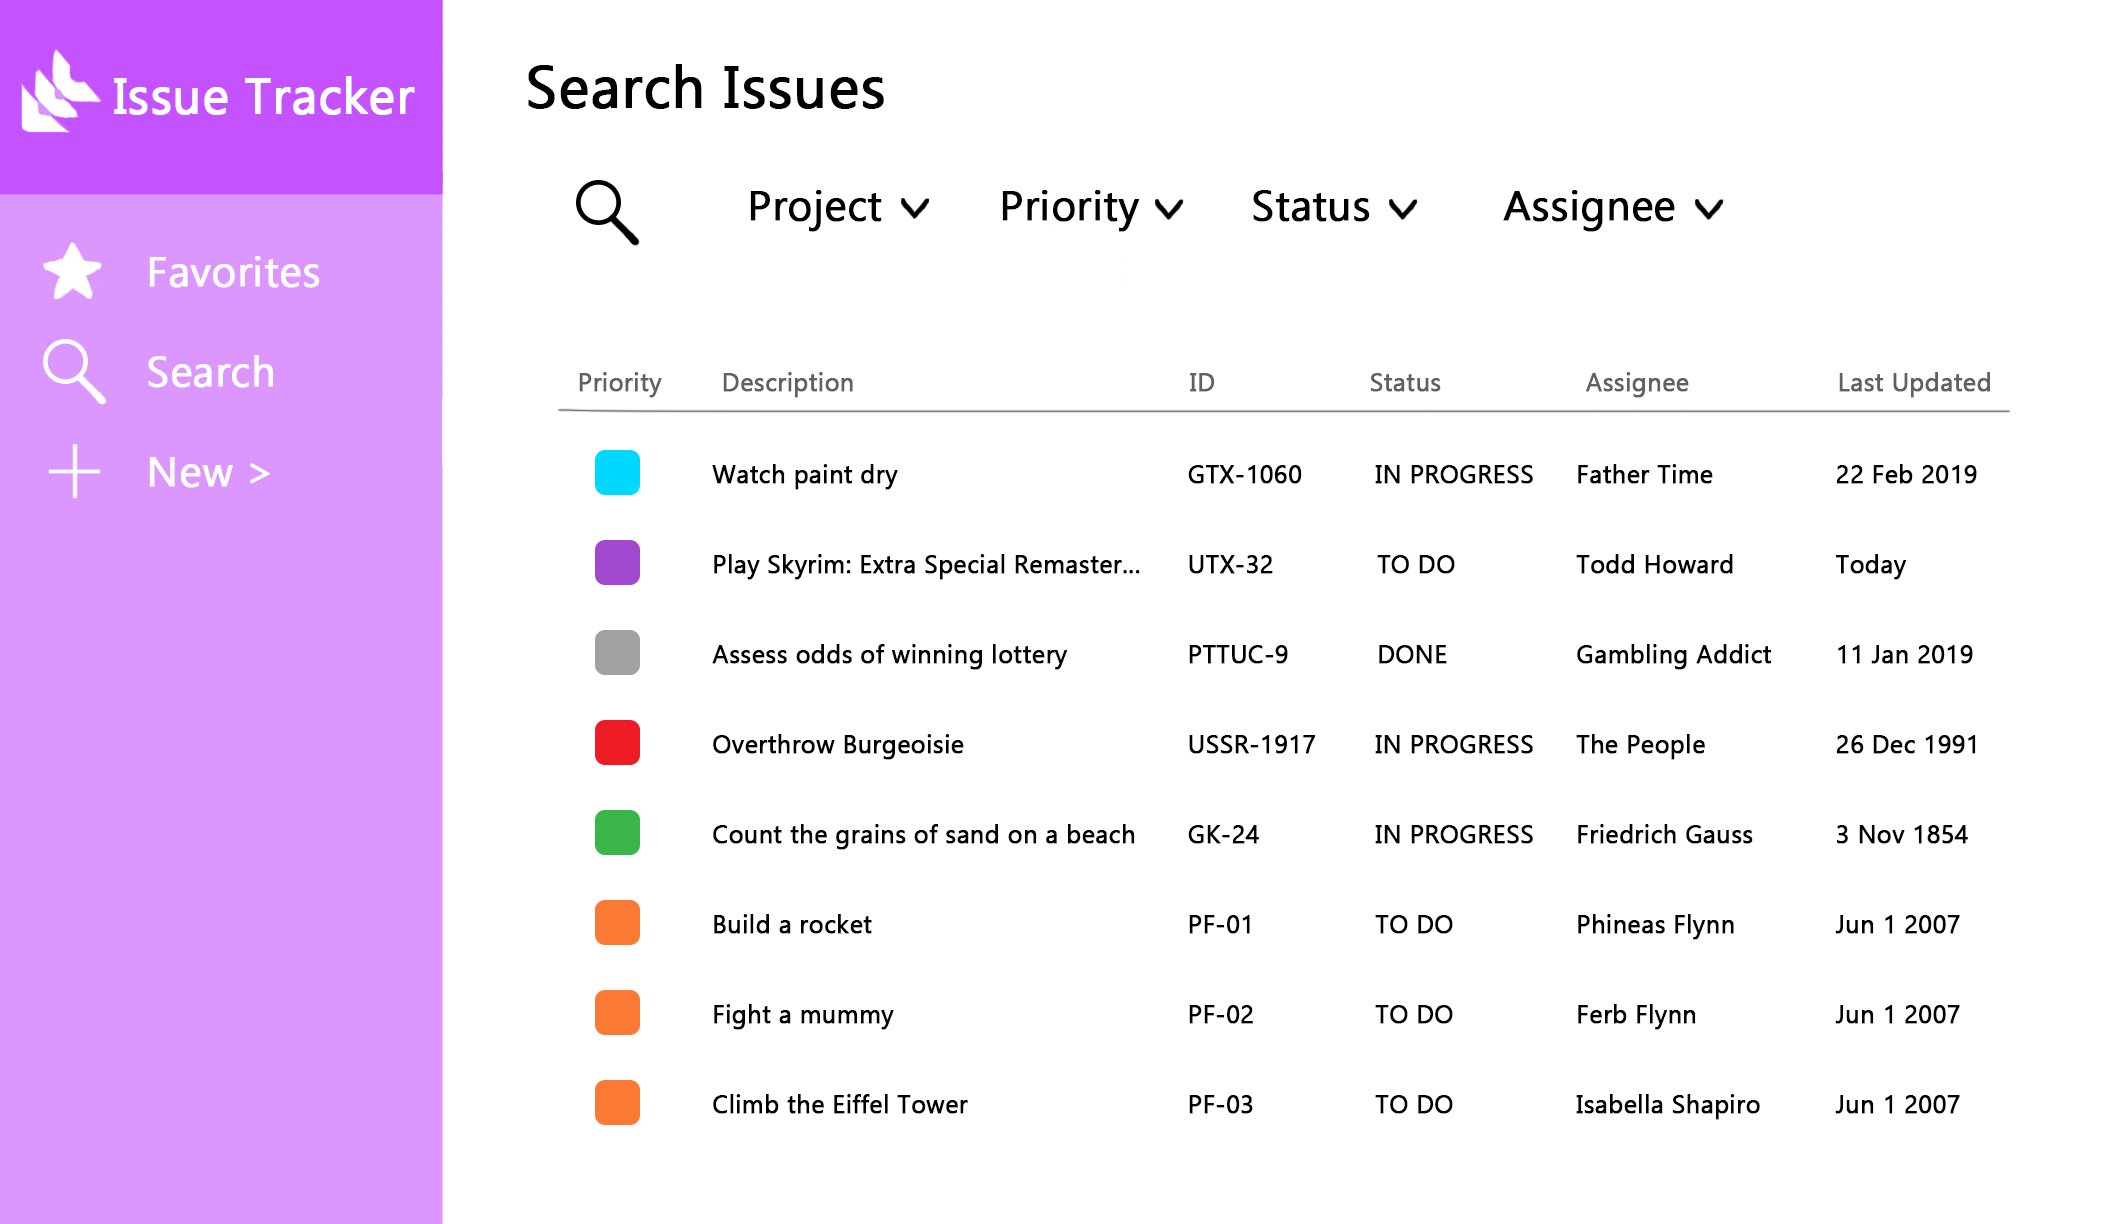
\includegraphics[scale=0.175]{IssueTrackerGUI_IssueList.png} }
    \fbox{ 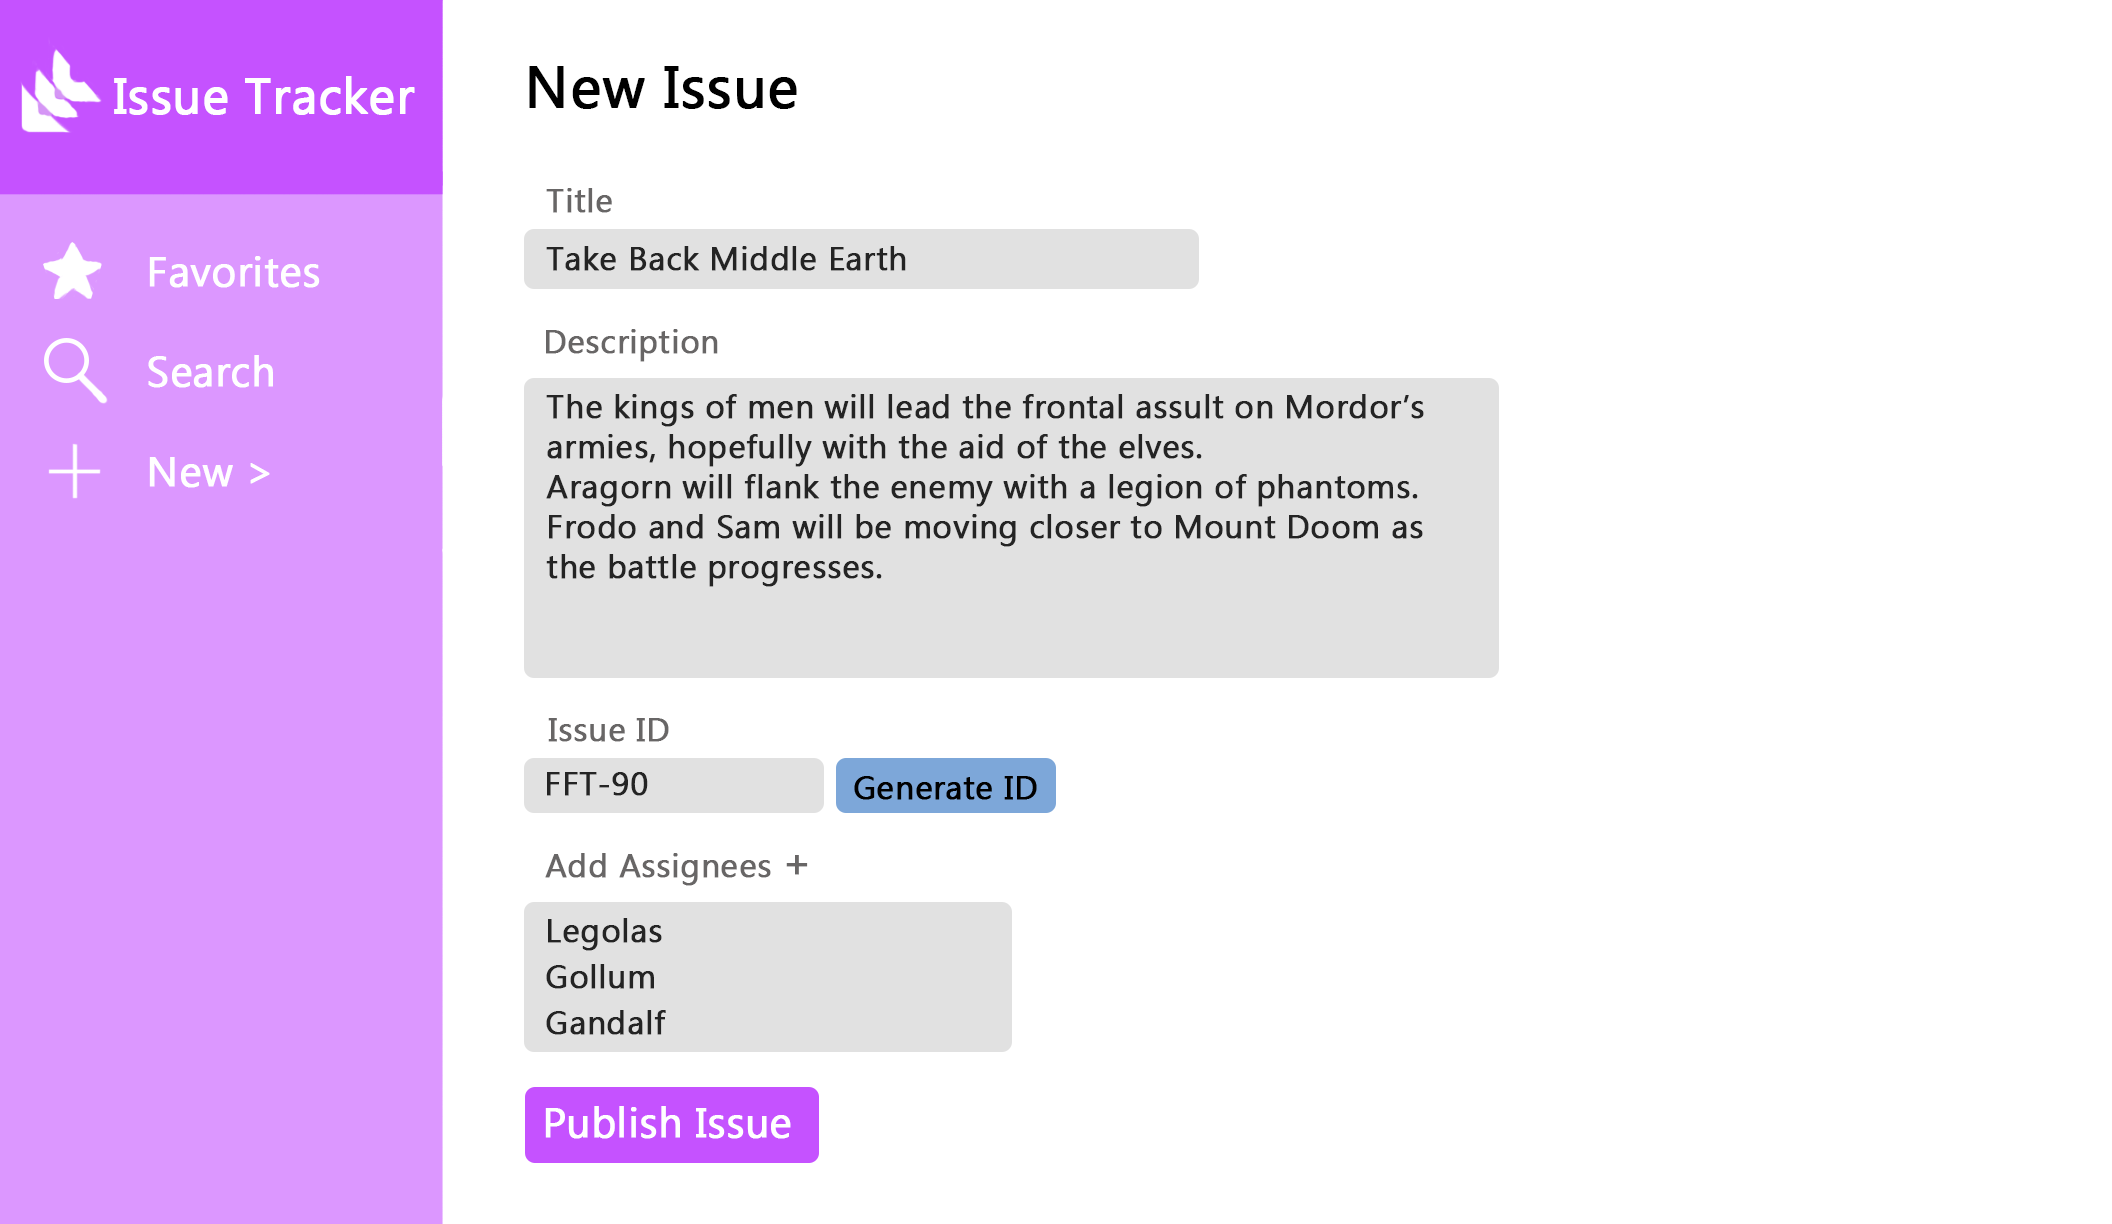
\includegraphics[scale=0.175]{IssueTrackerGUI_NewIssue.png} }

\section{Data Structure}

    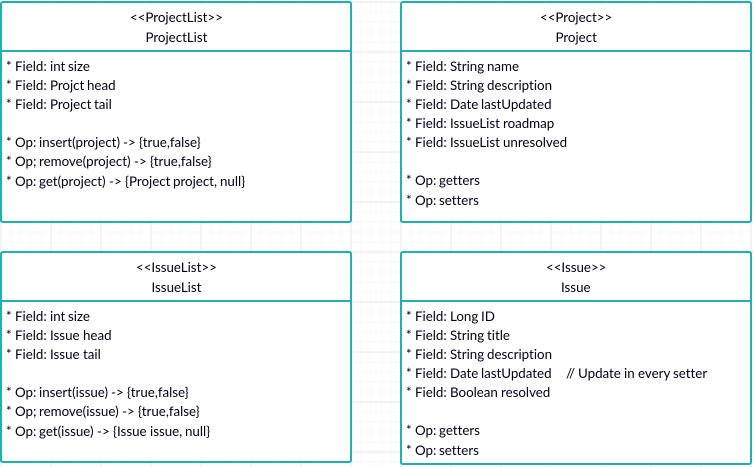
\includegraphics[scale=.6]{IssueTracker_UML.png}

\section{Input Data File Format}

    N/A

\section{Output Example}

    See GUI sketches

\section{Milestones}

    \subsection{Front End}

        \begin{itemize}
            \item Initialize Program
            \item Kill Program
            \item Deserializing JSON
            \item Add new Issue
            \item Edit existing Issue
            \item Remove Issue
            \item Represent fields of Issue
            \item Create new Project
            \item Edit existing Project
            \item Remove Project
        \end{itemize}

    \subsection{Back End}

        \begin{itemize}
            \item Build an Issue Object
            \item Build a list of Issues
            \item Build a Project Object
            \item Implement a list of Projects
            \item Writing to Database (JSON)
        \end{itemize}

\end{document}
